\section{Comparaison de différents modèle} \label{comparaison}

Nous avons mis en place un comparateur de différents modèle pour voir quel est le plus performant.
Pour cela nous avons essayé les 6 models ci-dessous afin de comparer leur accuracy.


\begin{center}
    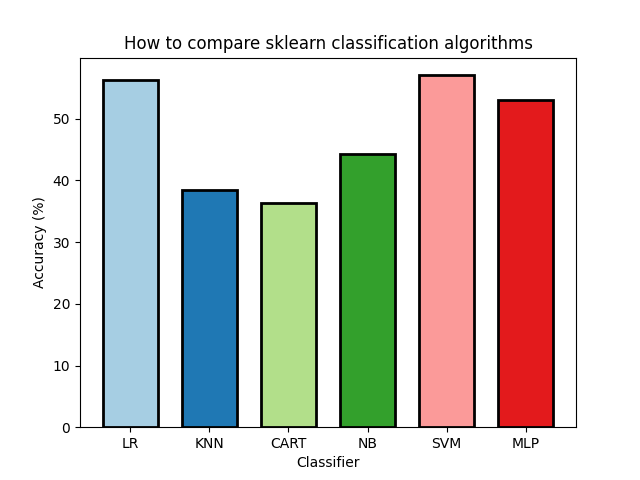
\includegraphics[scale=1]{graphs/compare_classifier.png}
    \captionof{figure}{Comparaison de différents modèles}
\end{center}

Les très meilleur semble être SVM, LogisticRegression et MLPClassifier. Les autres étant très éloigné nous avons décidé de tester uniquement ces trois méthodes.

\begin{center}
    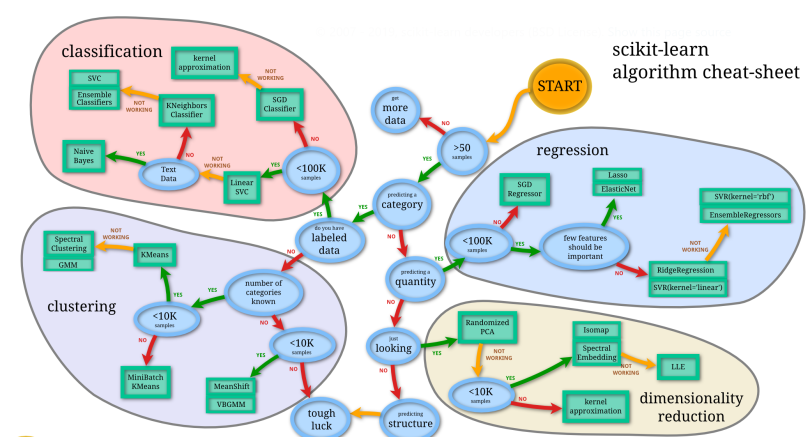
\includegraphics[scale=0.6]{img/sklearn-cheatsheet.png}
    \captionof{figure}{Roadmap pour le choix d'un modèle}
\end{center}

Nous nous sommes aussi appuyés sur l'image ci-dessus qui nous a aidé à choisir le meilleur modèle pour le projet que nous avons à faire en fonction des données. Puisque nous avons une base de données supérieur à 50 et inferieur à 100K et que nous classons du texte dans des catégories. Naturellement l'orientation s'est faite vers la classification avec le modèle LinearSVC.